\documentclass[a4paper,11pt]{paper}

% my packages
\usepackage[english]{babel}
\usepackage{graphicx}
\usepackage{verbatim}
\usepackage{appendix}
\usepackage{inputenc}
\usepackage{geometry}
%\usepackage{fullpage} % This is used to reduce the margins in the layout.
\usepackage{inputenc} % Package found in marco's
%\usepackage{rotating}
%\usepackage[small,anne]{caption}
\usepackage{caption}
\usepackage{amsmath}
\usepackage{makeidx}
\usepackage{listings} % code snippet :-)
\usepackage[pdftex]{hyperref}
\usepackage{url}
\usepackage{color} % To write in different colors


% General configuration
%\headheight 15pt
%\linespread{1.5}
%\bibliographystyle{unsrt}

% Hyperref configuration
%\renewcommand{\sectionautorefname}{Section}

\begin{document}

\pagestyle{plain} % to remove the header

% Cover
\thispagestyle{empty} % this removes the page number in the cover
\label{cover}

\begin{center}

{ \Huge
CSAtool
}

\vspace{5 mm}

{ \Large
User Guide
}

\vspace{10 mm}

\begin{figure}[h!]
	\centering
	
\includegraphics[scale=1.0]{pics/logo.png}
	\label{fig:logo}
\end{figure}

\vspace{20 mm}

{ \large
Created by:
\\ Stefano Brenna and Andrea Bonetti
\\ 
\href{mailto:crsaradctool@gmail.com}{\nolinkurl{crsaradctool@gmail.com}}

}



\end{center}


% Contents
\clearpage
\tableofcontents

% Body
\clearpage
\pagenumbering{arabic}
\label{intro}

\section{Introduction}
CSAtool is a MATLAB GUI simulation and modeling environment created for both the analysis and the assisted design of the capacitive DACs of charge-redistribution successive approximation analog-to-digital converters (CR SAR ADCs) in integrated-circuit technologies. In general, this tool allows to estimate both the static and the dynamic performance of such ADCs independently of the chosen technology.
This is possible simply providing models that allow the users to size the DAC array capacitive elements with an high degree of customization.
Moreover, the tool deals also with a variety of technological parameters which can be customized by the user to fit a particular technology performance.
By choosing a specific DAC topology defined by the combination of a capacitive network and a switching algorithm, sizing the capacitive array and setting the technology parameters, the effects of both intrinsic parasitic capacitances and capacitor mismatch on the ADC performance can be estimated.
In addition, with the aid of specific modules provided by the tool, also the impact  of the parasitic related to each critical array node and/or capacitor (for example the parasitic values coming from a post-layout c-extraction) can be analyzed. 
Finally, thanks to its simulation speed, which is up to a factor $10^5$ faster than those achievable with the most common EDA tools based testbenches, CSAtool offers the chance to perform statistical and montecarlo simulations over a desired number of realizations in a reasonable amount of time.

\label{howtorun}

\section{How to Run the Tool}
The steps to run the CSAtool on MATLAB are the following:
\begin{enumerate}
	\item Extract the folder of the CSAtool (/CSAtool) from the compressed file CSAtool.rar.
	\item Copy the extracted folder into your MATLAB folder (your desired work directory).
	\item Update the MATLAB search path with the new folder (be sure to operate in the directory containing the CSAtool folder).
	\item Type \texttt{CSAtool} in your MATLAB command window.
\end{enumerate}

\label{overview}

\section{Overview of the Tool}

CSAtool is a simulation environment based on capacitive network models tailored on each specific DAC topology. These models are based on vectors and matrix that reproduce the circuit proerties of a DAC topology. Given few parameters, among which the most important is the desired value of the unit capacitor ( the smallest compact capacitive element of the DAC), the tool produce a realization of a desired topology and evaluate its performance. In general the tool does NOT provide dedicated models of capacitors (MiMcaps, MoMcaps, PiPcaps...), but allows the designer to customize all the parameters which are necessary to model any of these options.

The main window of the tool, depicted in figure \ref{fig:main} presents the following sections:

\begin{figure}[h!]
	\centering
	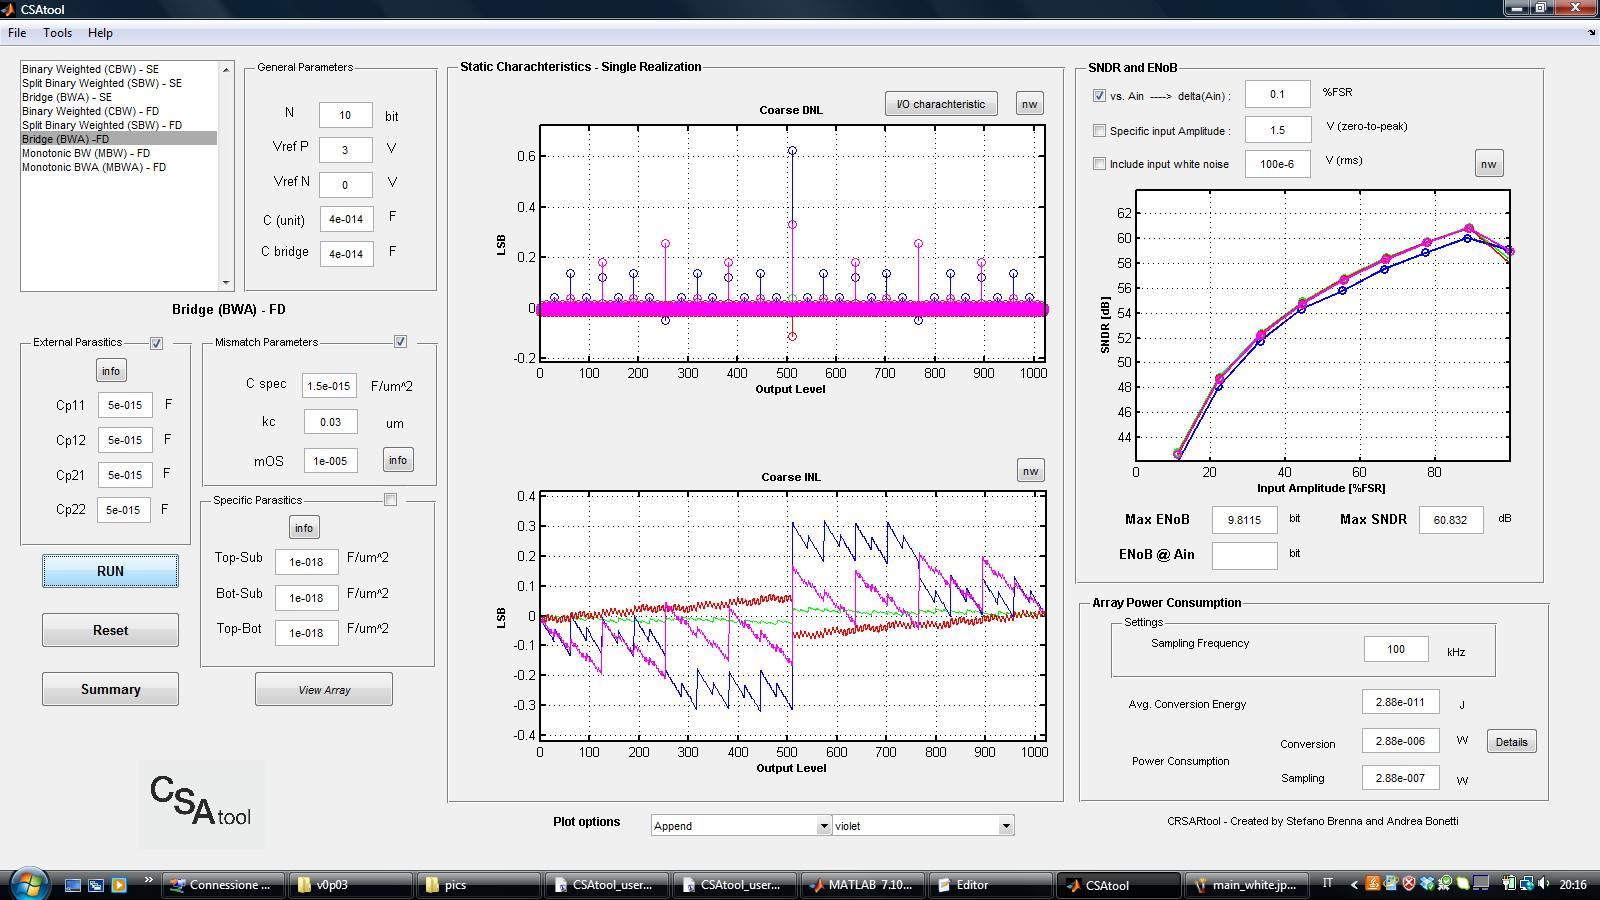
\includegraphics[scale=0.35]{pics/main_white.jpg}
	\caption{CSAtool main window.}
	\label{fig:main}
\end{figure}


\begin{description}

	\item[Topology] \hfill \\
	The topology of the CSAtool can be selected here among a list of the most common ones, at the top-left corner of the GUI main window. Both the array structure and the used switching scheme determine the topology. In addition, it is possible to choose either the single-ended (SE) or the fully-differential (FD) version. \\ The implemented models allow to choose among the following topologies:

\begin{itemize}
\item \texttt{Classic Binary Weighted - CBW (SE and FD)}: traditional binary weighted array combined to a traditional switching algorithm.
\item \texttt{Split Binary Weighted - SBW (SE and FD)}: binary weighted array where the MSB capacitor is split into a replica of the remaining part of the DAC, combined to the split capacitor array switching algorithm.
\item \texttt{Binary Weighted with Attenuation Capacitor BWA (SE and FD)}: simmetrical binary weighted array with attenuation capacitor combined to a traditional switching algorithm.
\item \texttt{Monotonic Binary Weighted MBW (intrinsically FD)}: traditional binary weighted array combined to a monotonic switching algorithm.
\item \texttt{Monotonic Binary Weighted with Attenuation Capacitor - MBWA (intrinsically FD)}: simmetrical binary weighted array with attenuation capacitor combined to a monotonic switching algorithm 
\end{itemize}

For additional information on the topologies and the switching schemes briefly described above, please refer to the papers listed in the section \emph{CSAtool Topologies References}.

	\item[General Parameters] \hfill \\
	General parameters section is located to the right of the topology selection list. The number of bits (N) , the input voltage range (difference between $V_{ref,P}$ and $V_{ref,N}$) and the nominal size of  the unit $C_{u}$ and the eventual attenuation capacitor $C_{b}$ can be arbitrarily set here. 

	\item[Mismatch Parameters] \hfill \\
          Each element of the capacitive DAC can be defined as the sum of its nominal value, which is a power of 2 multiple of the unit element, a mismatch contribution and the related parasitic. To contain the mismatch, in real DACs each capacitive bank of the array is typically implemented as the parallel of a desired number of unit capacitors.
 For this reason the mismatch contribution is here expressed and modeled as the sum of the mismatch of each unit element. Mismatch is absumed to be normally distributed with a zero-mean and a standard deviation which depends on the Pelgrom coefficient $k_{c}$ and the specific capacitance $C_{spec}$.

	The parameter \texttt{Cspec} is specific capacitance and it is defined as follows:
\begin{equation}
	C_{spec} = {C \over {W_{C} L_{C}}}
\end{equation}
\noindent Where $W_{C}$ and $L_{C}$ are respectively the width and the length of the unit capacitor whose value is $C$. Moreover, the parameter \texttt{kc} can be obtained from the following equation:
\begin{equation}
	\sigma \left ({\Delta C \over C} \right ) = k_{C} \sqrt{W_{C} L_{C}} + m_{OS}
\end{equation}
\noindent Where $\sigma \left ({\Delta C \over C} \right )$ is the standard deviation of the difference $\Delta C$ of identically designed capacitors, normalized to their absolute value $C$. The parameter $m_{OS}$ is given by the technology.
To enable the mismatch effect estimation, the checkbox related section of the main window must be checked.
\begin{figure}[h!]
	\centering
	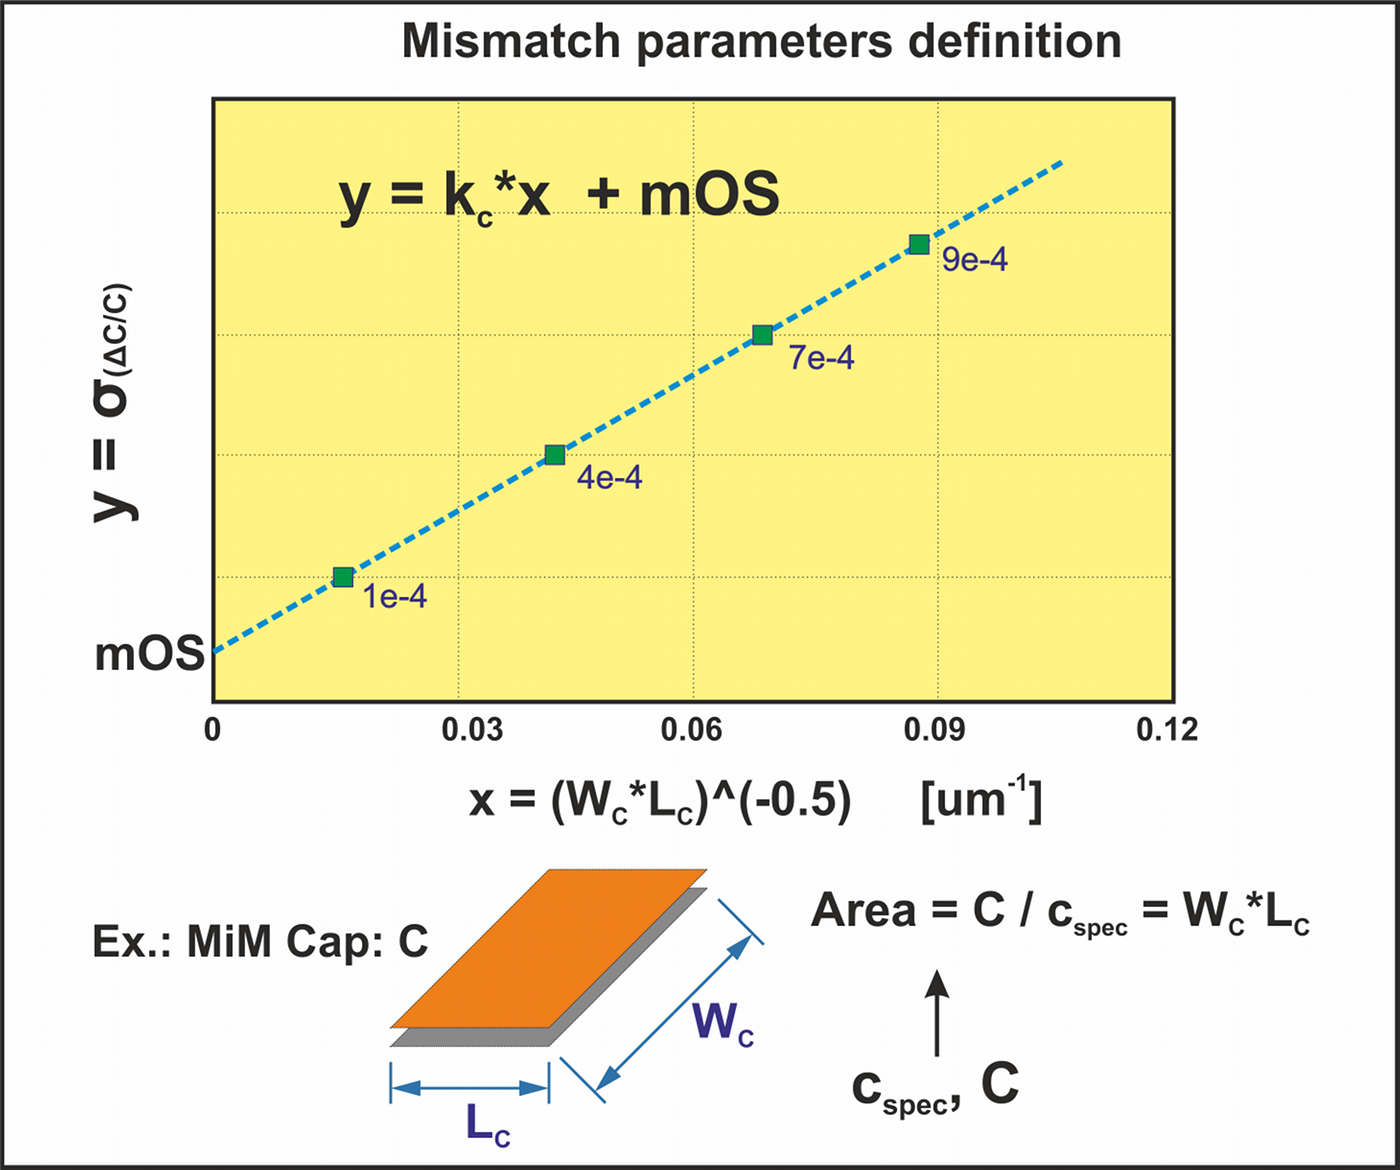
\includegraphics[scale=0.8]{pics/mismatch.png}
	\caption{Definition of the parameters for the mismatch of the capacitors.}
	\label{fig:mismatch}
\end{figure}

\item[Intrinsic Parasitics] \hfill \\
           It is possible to add the values of  intrinsic parasitic capacitances that are connected from the top-plate of the designed array (or sub-arrays) to the substrate, and from the the top-plate to the bottom-plate of every unit capacitor used to compose each capacitive bank of the DAC. The area-dependent parasitic capacitances to specify are the ones connected from the top plate of the capacitor to the substrate (Top-Sub), from the bottom plate of the capacitor to the substrate (Bot-Sub) and from the top plate to the bottom plate of the capacitor (Top-Bot).
This functionality is provided to give the designer the chance to evaluate the impact of those parasitics which are intrinsic of a particular class of capacitor and depend on its area, which is fixed by its size and specific capacitance.

\begin{figure}[h!]
	\centering
	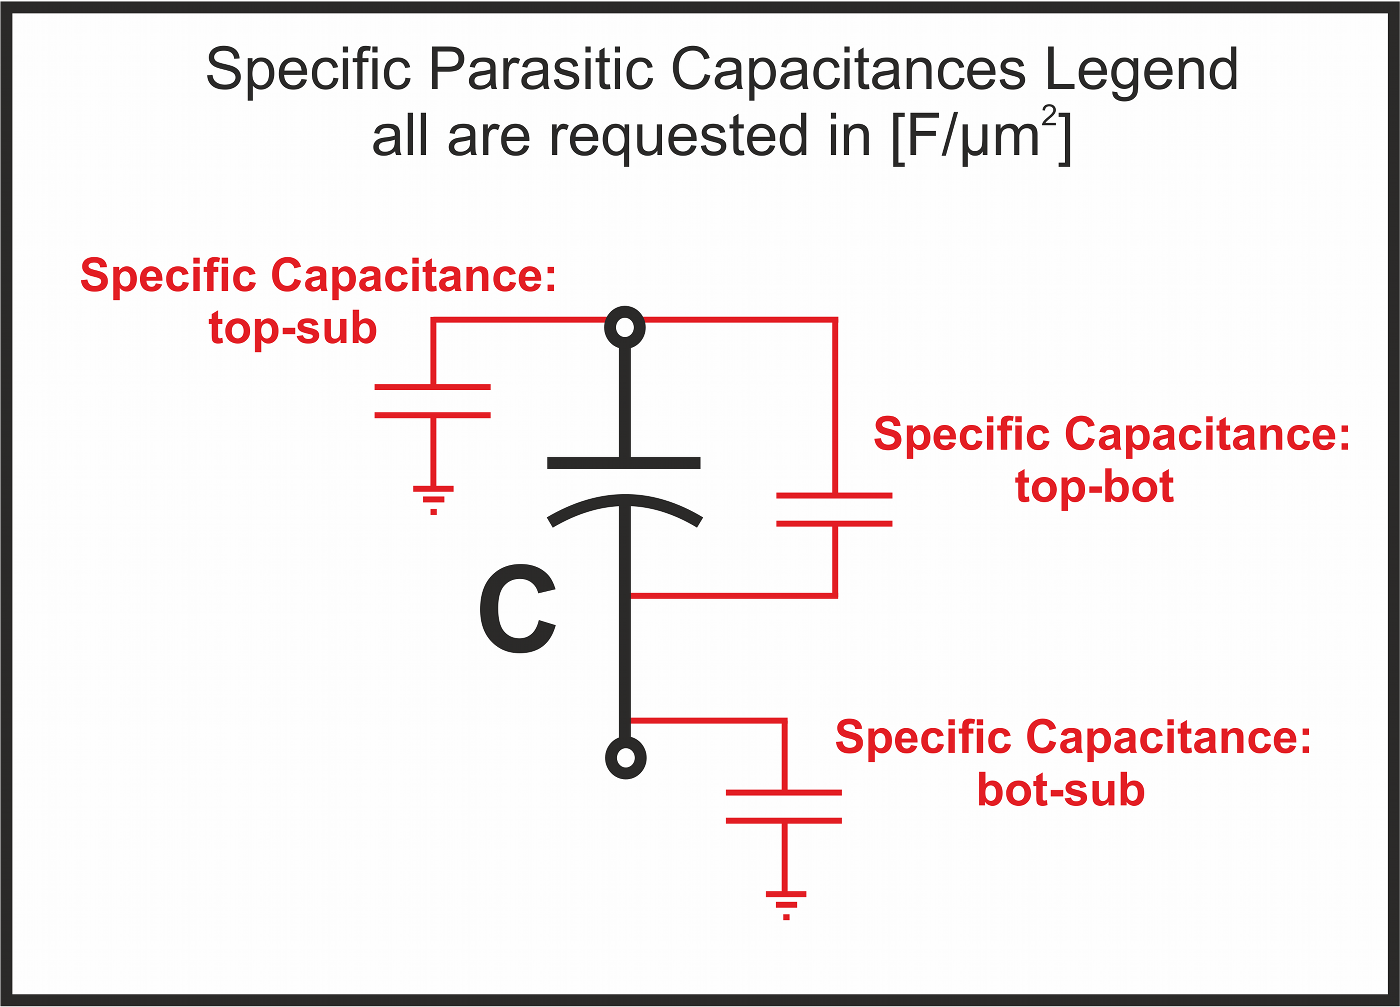
\includegraphics[scale=0.5]{pics/specpar.png}
	\caption{Specific parasitic capacitances.}
	\label{fig:specpar}
\end{figure}

Once again, it is worth noting here that in general the tool does NOT provide dedicated models of capacitors (MiMcaps, MoMcaps, PiPcaps...), but allows the designer to customize all the parameters which are necessary to model them. To enable the intrinsic parasitic effect estimation, the checkbox related section of the main window must be checked.

	\item[External Parasitics] \hfill \\
	The values of the external parasitic capacitances affecting the top plate node of DAC can be added here. The parasitic capacitances to specify are the ones connected from the top plate of the capacitive DAC and eventual sub-DACs to the substrate or to any fixed voltage node (for example $VDD$, $VSS$ or $V_{ref,P}$ and $V_{ref,N}$, if they don't coincide).\texttt{Cp11},\texttt{Cp12},\texttt{Cp21} and \texttt{Cp22} are the values that can be set in the most general case, depicted in figure \ref{fig:viewcpar}. If you have any doubt about the nodes affected by these parasitics, you can press the \texttt{View Array} button: an illustration will help you. 
	
\begin{figure}[h!]
	\centering
	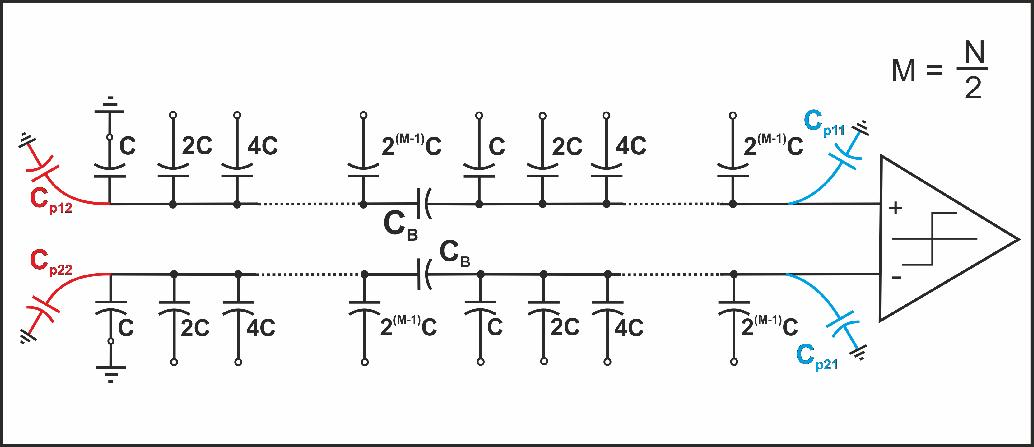
\includegraphics[scale=0.35]{pics/viewpar.jpg}
	\caption{External parasitic capacitances for a fully differential BWA.}
	\label{fig:viewcpar}
\end{figure}
	
To enable the external parasitic effect estimation, the checkbox related section of the main window must be checked.

	\item[Static Characteristics - Single Realization] \hfill \\
	Both DNL and INL graphs of the ADC are shown here for a single realization, estimated each time you press the \texttt{Run} button. By selecting the \emph{append} plot option, successive realizations can be compared on the same graph. 

	\item[SNDR and ENoB] \hfill \\
	The dependency of the SNDR on the amplitude of the input signal is plotted here, in the top right section of the main window. 
To enable this estimation, you can check any of the first two box on the top left. The first box allows to evaluate the SNDR of the customized DAC by points as a function of the input amplitude. The amplitude has a fixed step set by the user in the \texttt{delta(Ain)} cell and expressed as fraction of the FSR (i.e. 0.1 means 10 points). Both maximum achievable ENoB and SNDR are reported. \\
Differently, the second box enables the evaluation of the ENoB at a given input amplitude.
To estimate the dynamic performance, the tools simulate a conversion of an input sinusoid sampled well over nyquist, according to the IO charachteristic of the converter, including the current realization mismatch and  parasitics. The FFT is then performed on the output to evaluate the desired spectral metrics.
This approach also allows to sum a desired input referred white noise, defined by its rms value. This option just models an input referred noise and do not deal directly with its possible sources (comparator, switches...).

\begin{figure}[h!]
	\centering
	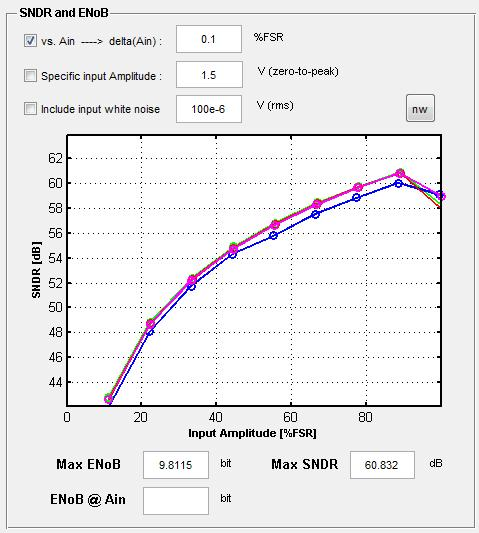
\includegraphics[scale=0.65]{pics/dynamic.jpg}
	\caption{Dynamic metrics estimation section.}
	\label{fig:dynamic}
\end{figure}

	\item[Array Power Consumption] \hfill \\
	By setting the sampling frequency of the ADC, it is possible to estimate the average energy required per conversion. The power consumptions of the conversion and of the sampling phase are also reported and include the impact of parasitics. \\ \textbf{This functionality is currently under development and could result  inaccurate for fully differential topologies.}
	
\end{description}
\label{addtools}

\section{Additional Tools}
For a further investigation of the static performances, it is possible to use additional tools. These can be selected by clicking on Tools, in the upper part of the CSAtool window.

\begin{description}

	\item[PPEX Tool] \hfill \\
	In case the extracted values of the parasitic capacitances are available from a post-layout analysis and/or if the user desired to investigate the effects produced by  localized parasitics, PPEX tool allows to add the value of the parasitic capacitance connected from the top plate to the bottom plate of each capacitive bank in the array. This is possible through the dedicated user interface shown in figure \ref{fig:ppex}. 

\begin{itemize}
\item Which is the difference between PPEX tool and the modules dedicated to \texttt{Specific Parasitics} and  \texttt{External Parasitics} that are already provided in CSAtool main window?
\end{itemize}

The external parasitics are just those connected from the top-plate of each eventual sub-DAC and the reference nets (substrate, VDD, GND ...).The specific parasitics are top-to-substrate (or reference nets), top-to-bottom, and bottom-to-substrate (or reference nets) stray capacitances that affect in general each unit capacitor, thus also the capacitive banks since each of them is built by multiple unit capacitors. These capacitances are specific so they depend on the area of the unit capacitor and so of each bank; in general they are proportional to the capacitance. 
PPEXtool offers the chance to estimate the effect of all those parasitics connected from the top to the bottom of any of the capacitive banks, which are not directly dependent on the area but on other issues, for example the layout quality, which depends only on the designer ability. This can be the case of wiring parasitics. 
Once a parasitic set is loaded and applied, all the analysis available from CSAtool can be performed through the main window and the other modules.
It is worth noting here that \textbf{the parasitic loaded through PPEXtool sum to the others specified in the main window} and also to the mismatch effect. 

\begin{figure}[h!]
	\centering
	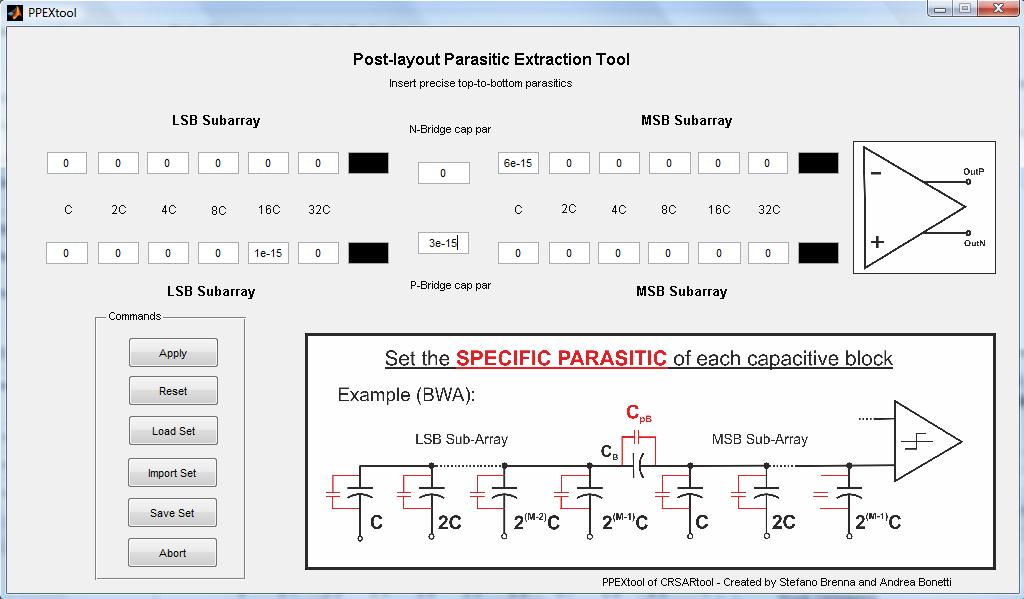
\includegraphics[scale=0.35]{pics/ppex.jpg}
	\caption{PPEX module for a 12-bit fully differential BWA.}
	\label{fig:ppex}
\end{figure}

	\item[SSA Tool] \hfill \\
	This tool provides a statistical analysis of the static performance over a desired number of runs, set by the parameter \texttt{Runs}. The parameter \texttt{sigma} act as a multiplier for the currently set pelgrom mismatch coefficient $k_{c}$. SSA tool output is represented by the standard deviation of DNL and INL as a function of the output code and by the distribution of their maximum absolute value.
\begin{figure}[h!]
	\centering
	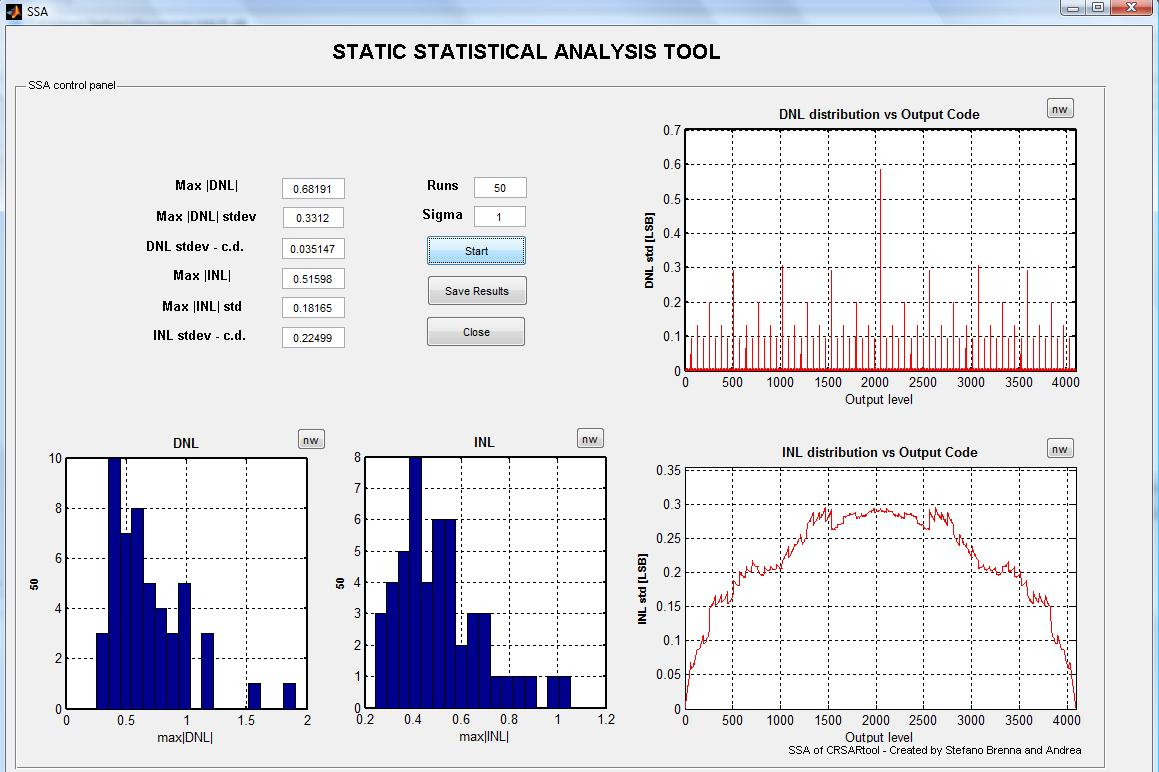
\includegraphics[scale=0.35]{pics/ssa.jpg}
	\caption{Static Statistical Analysis module.}
	\label{fig:ppex}
\end{figure}

	\item[ESA Tool] \hfill \\
	A statistical analysis of the achievable ENoB is presented here. The working principle is the same of SSAtool. The maximum ENoB distribution is evaluated over a desired number of runs, set by the parameter \texttt{Runs}. For each realization, the input amplitude of a virtual input sinusoid spans between the given minimum and maximum amplitudes, set by the users as a fraction of the FSR by defining the parameters \texttt{Minimum Input} and  \texttt{Minimum Input}.

\begin{figure}[h!]
	\centering
	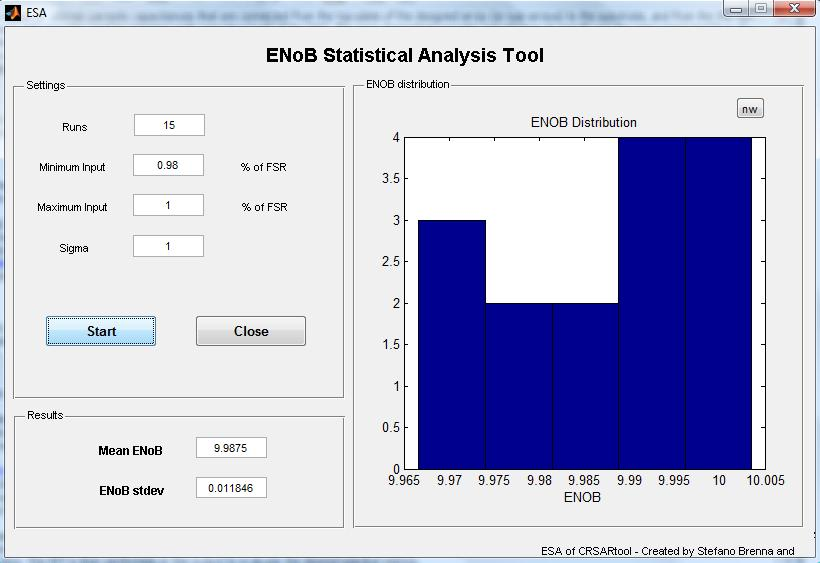
\includegraphics[scale=0.5]{pics/ESA.jpg}
	\caption{ESA module GUI.}
	\label{fig:esa}
\end{figure}



\end{description}
\label{topologies}

\section{CSAtool Topologies References}
The different CSAtool topologies reported in the tool are summarized here. For each of them, a document is given as reference for a better understanding.

\begin{flushleft} 
\begin{description}
	\item[Binary Weighted - CBW] \hfill \\
{ \footnotesize McCreary, J.L.; Gray, P.R.; , ``All-MOS charge redistribution analog-to-digital conversion techniques. I," \emph{Solid-State Circuits, IEEE Journal of} , vol.10, no.6, pp.371-379, Dec. 1975}

{ \footnotesize Suarez, R.E.; Gray, P.R.; Hodges, D.A.; , ``All-MOS charge-redistribution analog-to-digital conversion techniques. II," \emph{Solid-State Circuits, IEEE Journal of} , vol.10, no.6, pp.379-385, Dec. 1975}

	\item[Split Binary Weighted - SBW] \hfill \\
{ \footnotesize Ginsburg, B.P.; Chandrakasan, A.P.; , ``500-MS/s 5-bit ADC in 65-nm CMOS With Split Capacitor Array DAC," \emph{Solid-State Circuits, IEEE Journal of} , vol.42, no.4, pp.739-747, April 2007}

	\item[Binary Weighted with Attenuation Capacitor (Bridge) - BWA] \hfill \\
{ \footnotesize Agnes, A.; Bonizzoni, E.; Maloberti, F.; , ``Design of an ultra-low power SA-ADC with medium/high resolution and speed," \emph{Circuits and Systems, 2008. ISCAS 2008. IEEE International Symposium on} , vol., no., pp.1-4, 18-21 May 2008}

\item[Monotonic Binary Weighted - MBW] \hfill \\
{ \footnotesize Chun-Cheng Liu; Soon-Jyh Chang; Guan-Ying Huang; Ying-Zu Lin; , "A 10-bit 50-MS/s SAR ADC With a Monotonic Capacitor Switching Procedure," \emph{Solid-State Circuits, IEEE Journal of} , vol.45, no.4, pp.731-740, April 2010}

\item[Monotonic Binary Weighted with Attenuation Capacitor - MBWA] \hfill \\
{ \footnotesize S. Brenna; A. Bonfanti ; A. Abba; F. Caponio, A. L. Lacaita;  "Analysis and Optimization of a SAR ADC with Attenuation Capacitor" \emph{37th MIPRO Int. Conf. on Microelectronics} , May 2014}



%	\item[Split Bridge] \hfill \\

%	\item[Junction Splitting] \hfill \\
%{ \footnotesize Wenhuan Yu; Jiaming Lin; Temes, G.C.; , "Two-step junction-splitting SAR analog-to-digital converter," \emph{Circuits and Systems (ISCAS), Proceedings of 2010 IEEE International Symposium on} , vol., no., pp.1448-1451, May 30 2010-June 2 2010}


%	\item[Monotonic Binary Weigthed] \hfill \\
%{ \footnotesize Chun-Cheng Liu; Soon-Jyh Chang; Guan-Ying Huang; Ying-Zu Lin; , "A 10-bit 50-MS/s SAR ADC With a Monotonic Capacitor Switching Procedure," \emph{Solid-State Circuits, IEEE Journal of} , vol.45, no.4, pp.731-740, April 2010}

\end{description}
\end{flushleft} 
\label{contacts}

\section{Contacts}
For further information about the software, please contact: \href{mailto:crsaradctool@gmail.com}{\nolinkurl{crsaradctool@gmail.com}}
\label{authors}

\section{Authors}
The CSAtool has been created by:

\vspace{3 mm}

\noindent \textsc{Stefano Brenna}

\noindent PhD Candidate, Politecnico di Milano.

\vspace{3 mm}

\noindent \textsc{Andrea Bonetti}

\noindent Phd Candidate, EPFL.

\clearpage
\label{acknowledgments}

\section*{Acknowledgments}
This project would not have been possible without the support of many people. Therefore, we would like to thank:

\vspace{3 mm}

\noindent Andrea Lacaita, Andrea Bonfanti.

\noindent Microelectronics Laboratory, Politecnico di Milano.

\vspace{3 mm}

\noindent Andreas Hierlemann, Yihui Chen.

\noindent Bio Engineering Laboratory, ETH Zurich.

\vspace{3 mm}

\noindent Pascal Meinerzhagen.

\noindent Intel Labs.


\end{document}





